% !TEX root = ../intro-stellar-physics.tex

We saw in chapter~\ref{ch.basic-stellar-properties} that the equilibrium central temperature of a self-gravitating object---such as a star---with an ideal gas EOS depends \emph{solely} on the mass, radius, and composition of that star. For the Sun, this temperature is $\approx \val{15}{\Mega\K}$ and much higher than the surface effective temperature $T_{\!\mathrm{eff,\odot}} = \val{5780}{\K}$. The photons emitted from the Sun are coming from the cooler surface layers.

\newthought{Photons in a plasma, such as in the interior of the sun, transport energy.}  Were the sun transparent, these photons would immediately stream out, and the sun would release its stored energy in a fiery blast.  This doesn't happen: a photon can only travel a short distance before being scattered or absorbed. The net effect is that radiation generated in the core must travel a tortuous path, rather like a pinball, before reaching the surface and escaping.

\section{Interaction of radiation and matter}\label{s.interaction-radiation-matter}

How far does a photon---or any particle, for that matter---travel, on average, in the interior of the sun? Imagine a particle traveling with speed $v$.  Draw a cylinder, of length $\ell$ and cross-sectional area $\mathcal{A}$, around its future path, as shown in Fig.~\ref{f.MFP}. What the particle ``sees'' is that the cylinder is partly blocked by obstacles---other particles in its path. What is the probability of our particle making it through the cylinder unscathed?

\begin{marginfigure}
    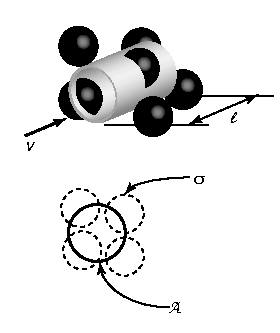
\includegraphics[width=\linewidth]{mean-free-path}
    \caption{\label{f.MFP} Schematic of a particle incident on a group of particles.}
\end{marginfigure}

The probability of the particle making it through is the ratio
\[
    \mathcal{P} = \frac{\textrm{total area covered by obstacles}}{\textrm{area of cylinder}}
\]
Denote the cross-sectional area of the other particles by $\sigma$.  If the density of obstacles is $n$, then the number of obstacles in the cylinder is $n\times(\mathcal{A}\ell)$, and therefore the fraction of the area blocked by the obstacles is
\begin{equation}
    \mathcal{P} = \frac{n\times(\mathcal{A}\ell)\times\sigma}{\mathcal{A}} = n\sigma\ell.
\label{e.prob-MFP}
\end{equation}
\marginnote{We are taking $\ell$ and $\mathcal{A}$ sufficiently small that we don't have to worry about particles overlapping.}
The particle will suffer a collision when $\mathcal{P}\to 1$, or when
\begin{equation}\label{e.MFP}
    \ell = \frac{1}{n\sigma}.
\end{equation}
We call $\ell$ the ``mean free path''.

\begin{exercisebox}[Mean free path for electron scattering]
    In the sun, free electrons scatter photons, and the cross-section is
    \[
    \sigma_{\mathrm{Th}} = \left(\frac{8\pi}{3}\right)\left(\frac{e^2}{m_e c^2}\right)^2 = \val{\sci{6.65}{-27}}{\meter^2}.
    \]
    What is the mean free path against this process for a photon?
\end{exercisebox}

\begin{exercisebox}[Mean free path of a hockey puck]\label{ex.MFP-2D}
    Suppose we have a flat surface on which pucks are sliding around, as shown in Fig.~\ref{f.MFP-2D} (Think of an air hockey table). The pucks bounce off the walls as they slide around.  Suppose there are $N$ pucks, each with a unit diameter, and the table is square with sides of length $L$.  Estimate the mean free path of a puck.
\end{exercisebox}

\begin{marginfigure}[-5\baselineskip]
    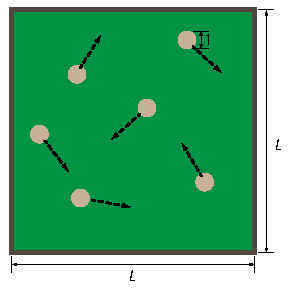
\includegraphics[width=\linewidth]{air-hockey-mfp}
    \caption[Mean free path of a hockey puck]{\label{f.MFP-2D}Schematic for Exercise~\ref{ex.MFP-2D}}
\end{marginfigure}


\section{Diffusion}\label{s.diffusion}

In the presence of scattering or absorption, the photons crossing the face can travel one mean free path $\ell$. Imagine a small cube with sides of length $\ell$ and filled with photons. The total radiant energy in the cube is $\Delta E$. In a time $\Delta t = \ell/c$, all of the energy will leave this cube. The total luminosity is $\Delta E/\Delta t = c\Delta E/\ell$. If everything is isotropic, then the flux out of any one face is $1/6$ of the luminosity, divided by the area of that face:
\[
	F = \frac{1}{6\ell^{2}}\frac{c\Delta E}{\ell} = \frac{1}{6}c U,
\]
where $U = E/\ell^{3}$ is the radiative energy density. 

\begin{marginfigure}
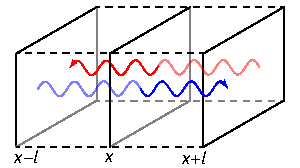
\includegraphics[width=\linewidth]{diffusive-flux}
\caption{\label{f.diffusive-flux} Illustration of net flux crossing a face between regions with slightly different energy densities.}
\end{marginfigure}
Now place two of these cubes against one another, with their common face located at position $x$. The energy density of the two cubes need not be the same; the energy density of the left cube is $U(x-\ell)$ and of the right cube is $U(x+\ell)$ (see Fig.~\ref{f.diffusive-flux}). The net flux traveling in the $x$-direction through the common face is then
\[
	F = {\color{blue}\frac{1}{6} c U(x-\ell)} - {\color{red}\frac{1}{6} c U(x+\ell)} \approx -\frac{1}{3}c\ell \DDx{U}.
\]
This is an expression for a \textbf{diffusive flux}. Although we gave a heuristic explanation, the formula is in general true:
\begin{eqnarray}
\nonumber
(\textrm{flux of something}) &=& -\frac{1}{3}\times(\textrm{speed of carriers})\times(\textrm{MFP of carriers})\\
&&\times \grad(\textrm{density of something})
\label{e.diffusive-flux}
\end{eqnarray}
For radiation, the ``something'' is ``radiative energy'' and the carriers are photons.

\newthought{Relate to random walk}


